%%%%%%%%%%%%%%%%%%%%%%%%%%%%%%%%%%%%%%%%%
% Short Sectioned Assignment LaTeX Template Version 1.0 (5/5/12)
% This template has been downloaded from: http://www.LaTeXTemplates.com
% Original author:  Frits Wenneker (http://www.howtotex.com)
% License: CC BY-NC-SA 3.0 (http://creativecommons.org/licenses/by-nc-sa/3.0/)
%%%%%%%%%%%%%%%%%%%%%%%%%%%%%%%%%%%%%%%%%

%----------------------------------------------------------------------------------------
%	PACKAGES AND OTHER DOCUMENT CONFIGURATIONS
%----------------------------------------------------------------------------------------

\documentclass[paper=a4, fontsize=11pt]{scrartcl} % A4 paper and 11pt font size

% ---- Entrada y salida de texto -----

\usepackage[T1]{fontenc} % Use 8-bit encoding that has 256 glyphs
\usepackage[utf8]{inputenc}

% ---- Idioma --------

\usepackage[spanish, es-tabla]{babel} % Selecciona el español para palabras introducidas automáticamente, p.ej. "septiembre" en la fecha y especifica que se use la palabra Tabla en vez de Cuadro

% ---- Otros paquetes ----

\usepackage{amsmath,amsfonts,amsthm} % Math packages
\usepackage{graphics,graphicx, floatrow} %para incluir imágenes y notas en las imágenes
\usepackage{graphics,graphicx, float} %para incluir imágenes y colocarlas
\usepackage{hyperref} % url in references

% Para hacer tablas comlejas
\usepackage{multirow}
\usepackage{threeparttable}

\usepackage{fancyhdr} % Custom headers and footers
\pagestyle{fancyplain} % Makes all pages in the document conform to the custom headers and footers
\fancyhead{} % No page header - if you want one, create it in the same way as the footers below
\fancyfoot[L]{} % Empty left footer
\fancyfoot[C]{} % Empty center footer
\fancyfoot[R]{\thepage} % Page numbering for right footer
\renewcommand{\headrulewidth}{0pt} % Remove header underlines
\renewcommand{\footrulewidth}{0pt} % Remove footer underlines
\setlength{\headheight}{13.6pt} % Customize the height of the header

\numberwithin{equation}{section} % Number equations within sections (i.e. 1.1, 1.2, 2.1, 2.2 instead of 1, 2, 3, 4)
\numberwithin{figure}{section} % Number figures within sections (i.e. 1.1, 1.2, 2.1, 2.2 instead of 1, 2, 3, 4)
\numberwithin{table}{section} % Number tables within sections (i.e. 1.1, 1.2, 2.1, 2.2 instead of 1, 2, 3, 4)

\setlength\parindent{0pt} % Removes all indentation from paragraphs - comment this line for an assignment with lots of text

\newcommand{\horrule}[1]{\rule{\linewidth}{#1}} % Create horizontal rule command with 1 argument of height

\usepackage{textcomp}
\usepackage{hyperref}

%----------------------------------------------------------------------------------------
%	DATOS
%----------------------------------------------------------------------------------------

\newcommand{\myName}{Francisco Javier Bolívar Lupiáñez}
\newcommand{\myDegree}{Máster en Ingeniería Informática}
\newcommand{\myFaculty}{E. T. S. de Ingenierías Informática y de Telecomunicación}
\newcommand{\myDepartment}{Ciencias de la Computación e Inteligencia Artificial}
\newcommand{\myUniversity}{\protect{Universidad de Granada}}
\newcommand{\myLocation}{Granada}
\newcommand{\myTime}{\today}
\newcommand{\myTitle}{Práctica 1}
\newcommand{\mySubtitle}{Despliegue de MVs y Aplicaciones Web}
\newcommand{\mySubject}{Cloud Computing: Servicios y Aplicaciones}
\newcommand{\myYear}{2016-2017}

%----------------------------------------------------------------------------------------
%	PORTADA
%----------------------------------------------------------------------------------------


\title{	
	\normalfont \normalsize 
	\textsc{\textbf{\mySubject \space (\myYear)} \\ \myDepartment} \\[20pt] % Your university, school and/or department name(s)
	\textsc{\myDegree \\[10pt] \myFaculty \\ \myUniversity} \\[25pt]
	\horrule{0.5pt} \\[0.4cm] % Thin top horizontal rule
	\huge \myTitle: \mySubtitle \\ % The assignment title
	\horrule{2pt} \\[0.5cm] % Thick bottom horizontal rule
	\normalfont \normalsize
}

\author{\myName} % Nombre y apellidos

\date{\myTime} % Incluye la fecha actual
%----------------------------------------------------------------------------------------
%	INDICE
%----------------------------------------------------------------------------------------

\begin{document}
	
\definecolor{light-gray}{gray}{0.95}
	
\lstset {
	basicstyle=\scriptsize,
	frame=single,
	backgroundcolor=\color{grey}
}
	
\setcounter{page}{0}

\maketitle % Muestra el Título
\thispagestyle{empty}

\newpage %inserta un salto de página

\tableofcontents % para generar el índice de contenidos

%\listoffigures

\newpage

%----------------------------------------------------------------------------------------
%	DOCUMENTO
%----------------------------------------------------------------------------------------

\section{Introducción}

El objetivo de esta práctica es familiarizarse con el uso de una plataforma IaaS y desarrollar habilidades de despliegue de máquinas virtuales y aplicaciones web sencillas.
\\ \\
Para ello el alumno deberá realizar las tareas que se describen a continuación usando la plataforma OpenNebula:

\begin{itemize}
	\item Crear dos MVs, cada una con una distribución de Linux:
	\begin{itemize}
		\item En la primera MV instalar y configurar un servidor web.
		\item En la segunda MV instalar y configurar un sistema gestor de bases de datos (SGBD).
	\end{itemize}
	\item Desarrollar una aplicación web sencilla alojada en la MV1, que use una base de datos manejada por el SGBD instalado en al MV2. La aplicación web debe incluir el uso de formularios y la consulta y modificación de datos almacenados en la BD.
	\item Realizar el despliegue de ambas MVs, para evaluar el funcionamiento de la aplicación.
\end{itemize}

\label{sec:conexion}
\subsection{Conexión con OpenNebula}

Para conectarse con OpenNebula hay que hacerlo mediante ssh conectándose a la dirección \texttt{docker.ugr.es} con el usuario \texttt{mccDNI-SIN-LETRA}. Por ejemplo:

\begin{lstlisting}
ssh mcc12345678@docker.ugr.es
\end{lstlisting}

Una vez conectado escribir la siguiente orden: 

\begin{lstlisting}
oneuser login mccDNI-sin-LETRA --ssh --force
\end{lstlisting}

Y con: 

\begin{lstlisting}
more .one/one\_auth
\end{lstlisting}

podemos obtener las credenciales para acceder a la plataforma desde la web \url{http://docker.ugr.es:9869}.

\section{Despliegue de máquinas virtuales}

El despliegue de máquinas virtuales se ha realizado mediante la interfaz de línea de órdenes de OpenNebula. Para ello hay que conectarse como se especificó en la sección \ref{sec:conexion}.

\label{sec:crear-plantilla}
\subsection{Crear plantilla}

Para crear una plantilla necesitamos información como el identificador de la imagen como la red propia del usuario.
\\ \\
Para encontrar el id de la imagen que se utilizará en la plantilla, listamos las imágenes disponibles con:

\begin{lstlisting}
oneimage list
\end{lstlisting}

\begin{figure}[H]
	\centering
	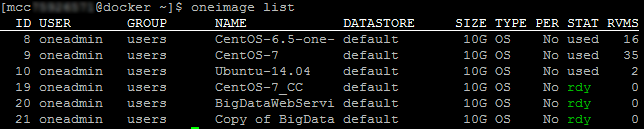
\includegraphics[width=14cm]{img/oneimage-list}
	\caption{Lista de imágenes disponibles}
	\label{fig:one-image-list}
\end{figure}

Y para dar con la red:

\begin{lstlisting}
onevnet list | grep mccDNI-SIN-LETRA
\end{lstlisting}

\begin{figure}[H]
	\centering
	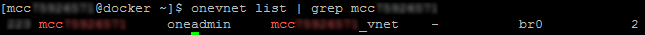
\includegraphics[width=14cm]{img/onevnet-list}
	\caption{Datos de red de un usuario específico}
	\label{fig:onevnet-list}
\end{figure}

Con estos datos ya podemos crear un template, por ejemplo:

\begin{lstlisting}
onetemplate create --name "Template_CentOS-6.5" --cpu 1 
--vcpu 1 --memory 1024 --arch x86_64 --disk 8 
--nic "MI-ID-RED" --vnc --ssh --net_context
\end{lstlisting}

Esto creará un template y le asignará un identificador único. Para consultarlo podemos listar nuestros templates con:

\begin{lstlisting}
onetemplate list
\end{lstlisting}

\begin{figure}[H]
	\centering
	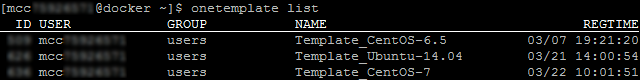
\includegraphics[width=14cm]{img/onetemplate-list}
	\caption{Lista de templates}
	\label{fig:onetemplate-list}
\end{figure}

\subsection{Desplegar máquina virtual}

Para crear una máquina virtual necesitaremos un template, cuyo ID podemos obtener como se ha explicado en la Sección \ref{sec:crear-plantilla}.
\\ \\
Tan solo hay que usar la orden:

\begin{lstlisting}
onetemplate instantiate ID
\end{lstlisting}

Esto instanciará e iniciará la máquina virtual pasando por distintos estados (Figura \ref{fig:grafo-estados}).

\begin{figure}[H]
	\centering
	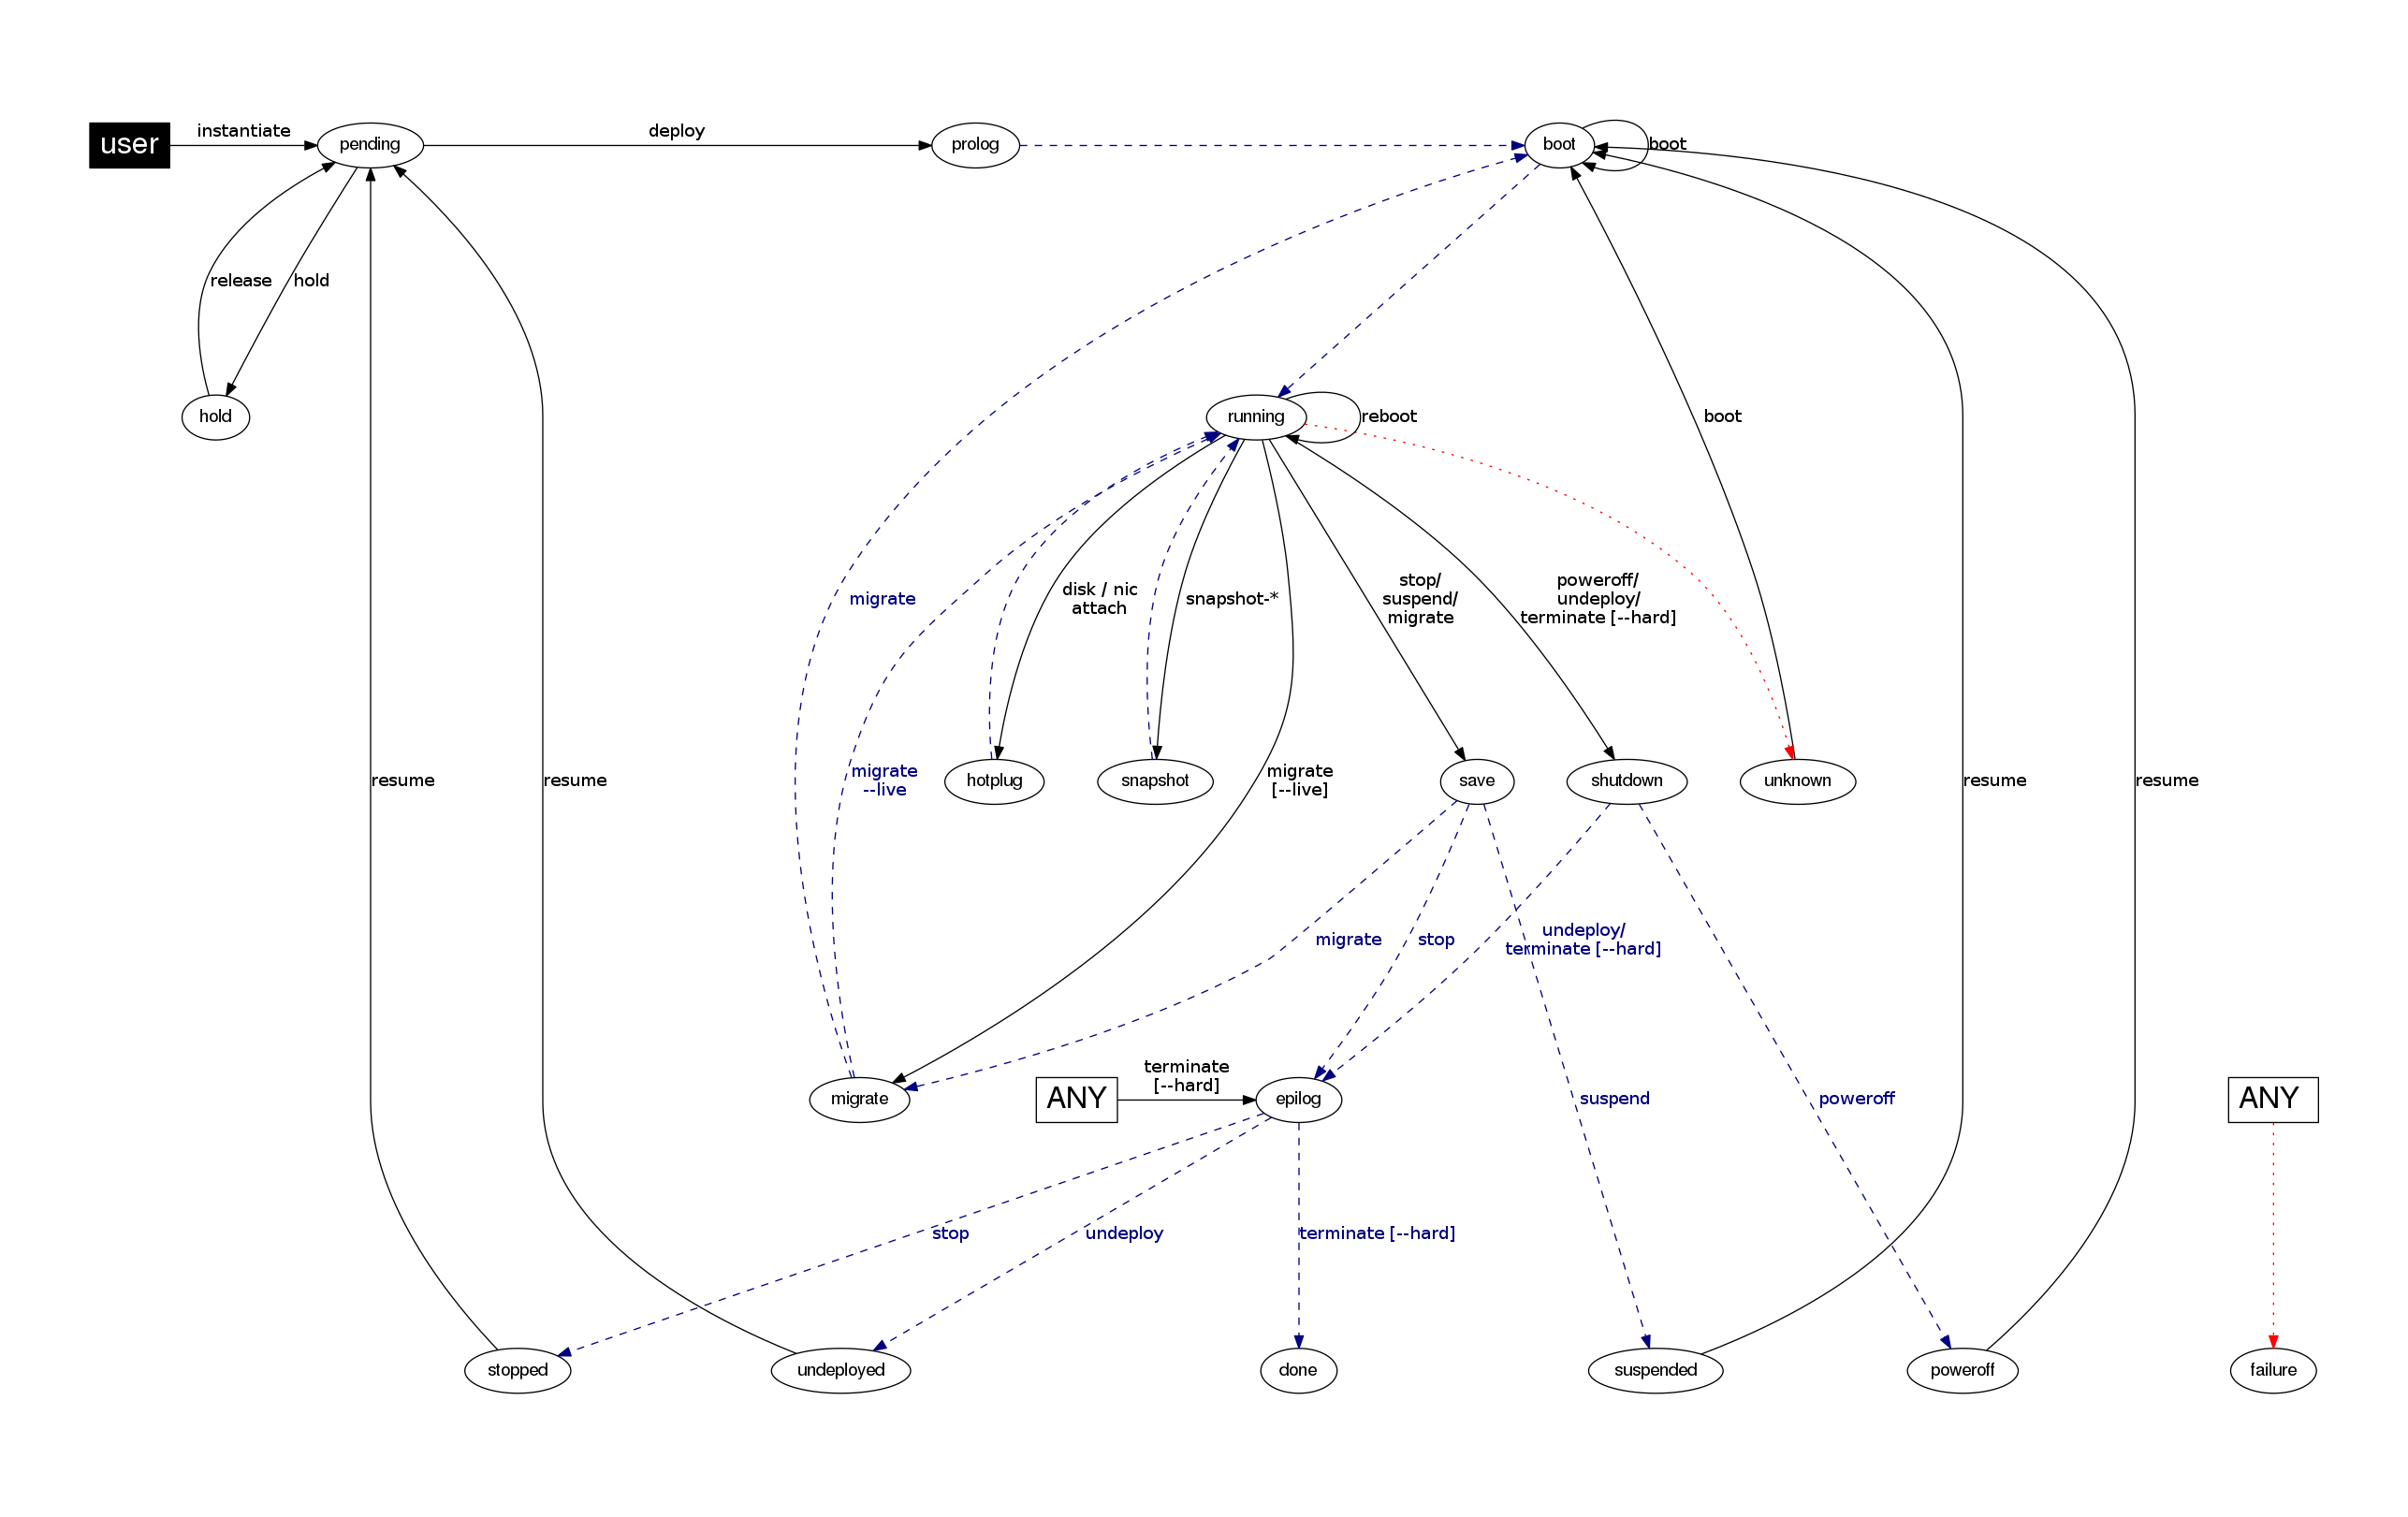
\includegraphics[width=14.5cm]{img/grafo-estados}
	\caption{Grafo de los estados por los que pasa una máquina virtual}
	\label{fig:grafo-estados}
\end{figure}

Para listar las máquinas virtuales usaremos:

\begin{lstlisting}
onevm list
\end{lstlisting}

\begin{figure}[H]
	\centering
	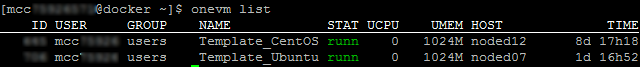
\includegraphics[width=14cm]{img/onevm-list}
	\caption{Lista de máquinas virtuales}
	\label{fig:onevm-list}
\end{figure}

La información de una máquina virtual específica la podemos consultar con:

\begin{lstlisting}
onevm show ID
\end{lstlisting}

De aquí podemos obtener la dirección IP (\texttt{ETH0\_IP}) para conectarse posteriormente a ella vía ssh:

\begin{figure}[H]
	\centering
	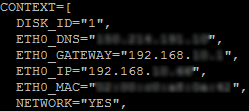
\includegraphics[width=5cm]{img/onevm-show-context}
	\caption{Direcciones de red de una máquina virtual}
	\label{fig:onevm-show-context}
\end{figure}

\section{Servidor web}

Usaremos la máquina virtual con Ubuntu 14.04 para alojar nuestro servidor web (Apache). Para ello seguiremos los pasos de un tutorial de DigitalOcean \cite{InstallLAMPUbuntu14.04} con los que instalaremos Apache y PHP e ignorando los pasos para instalar MySQL pues, recordamos, esta primera máquina virtual solo contendrá el servidor web.
\\ \\
Para comenzar nos conectamos a la máquina virtual mediante ssh con \texttt{ssh root@ETH0\_IP} y lo primero que haremos será actualizar el sistema con:

\begin{lstlisting}
apt-get update && apt-get upgrade
\end{lstlisting}

Ahora instalaremos Apache con:

\begin{lstlisting}
apt-get install apache2
\end{lstlisting}


Una vez instalado se puede lanzar usando:

\begin{lstlisting}
service apache2 restart
\end{lstlisting}

Por último instalamos PHP pues la aplicación web está desarrollada con esta tecnología. Para ello ejecutamos:

\begin{lstlisting}
apt-get install php5 libapache2-mod-php5 php5-mcrypt
\end{lstlisting}

Para darle prioridad a los fuentes en .php editamos el fichero \texttt{dir.conf} que se encuentra en el directorio \texttt{/etc/apache2/mods-enabled} colocando \texttt{index.php} el primero (justo por detrás de \texttt{DirectoryIndex}).
\\ \\
Una vez instalado podemos cargar los fuentes en el directorio \texttt{/var/www/html/}. Yo los he obtenido clonando mi repositorio de GitHub donde están alojados: \url{https://github.com/fblupi/starsator-web}.

\section{SGBD}

Usaremos la máquina virtual con CentOS 6.5 para alojar nuestro SGBD (MySQL). Para ello seguiremos los pasos de un tutorial de DigitalOcean \cite{InstallLAMPCentos6.5} con los que instalaremos MySQL ignorando los pasos para instalar Apache y PHP pues, recordamos, esta máquina virtual solo contendrá el SGBD.
\\ \\
Para comenzar nos conectamos a la máquina virtual mediante ssh con \texttt{ssh root@ETH0\_IP} y lo primero que haremos será actualizar el sistema con:

\begin{lstlisting}
yum update
\end{lstlisting}

Ahora instalaremos Apache con:

\begin{lstlisting}
yum install mysql-server
\end{lstlisting}

Una vez instalado se puede lanzar usando:

\begin{lstlisting}
service mysqld start
\end{lstlisting}

Una vez instalado podemos cargar la base de datos cargando el script que se encuentra en \url{https://github.com/fblupi/starsator-db} con la siguiente orden:

\begin{lstlisting}
mysql < stars.sql
\end{lstlisting}

\section{Conectar ambas máquinas virtuales}

\subsection{SGBD}

Lo primero que hay que hacer es abrir el puerto 80 en la máquina donde se aloja el SGBD y asignárselo a MySQL para poder acceder externamente al servicio.
\\ \\
Para ello hay que abrir el puerto usando \texttt{iptables} \cite{OpenPortIptables} usando la orden:

\begin{lstlisting}
iptables -I INPUT -p tcp -m tcp --dport 80 -j ACCEPT
service iptables save
\end{lstlisting}

A continuación hay que editar el fichero \texttt{my.cnf} que se encuentra en \texttt{/etc} y agregarle las líneas: 

\begin{lstlisting}
[client]
port=80
\end{lstlisting}

Y finalmente se reinicia el servicio: 

\begin{lstlisting}
service mysqld restart
\end{lstlisting}

%----------------------------------------------------------------------------------------
%	REFERENCIAS
%----------------------------------------------------------------------------------------

\newpage

\bibliography{referencias} %archivo referencias.bib que contiene las entradas 
\bibliographystyle{plain} % hay varias formas de citar

\end{document}